\documentclass[10pt]{article} % base size; all font sizes are redefined below for A0 scale

% ==============================================================================
% PACKAGES
% ==============================================================================
\usepackage[a0paper, portrait, margin=2.5cm]{geometry}
\usepackage{multicol}
\usepackage{xcolor}
\usepackage[most]{tcolorbox}
\usepackage{tikz}
\usetikzlibrary{positioning, arrows.meta, shapes.geometric, calc}
\usepackage{pgfplots}
\pgfplotsset{compat=1.18}
\usepackage{amsmath, amssymb}
\usepackage{booktabs}
\usepackage{array}
\usepackage{microtype}
\usepackage[shortlabels]{enumitem}
\usepackage{times}

% ==============================================================================
% POSTER FONT SIZES  (scaled for A0 paper, approximately 2× standard article)
% ==============================================================================
\renewcommand{\normalsize}  {\fontsize{22pt}{28pt}\selectfont}
\renewcommand{\small}       {\fontsize{18pt}{23pt}\selectfont}
\renewcommand{\footnotesize}{\fontsize{15pt}{19pt}\selectfont}
\renewcommand{\scriptsize}  {\fontsize{12pt}{16pt}\selectfont}
\renewcommand{\large}       {\fontsize{27pt}{33pt}\selectfont}
\renewcommand{\Large}       {\fontsize{32pt}{39pt}\selectfont}
\renewcommand{\LARGE}       {\fontsize{38pt}{46pt}\selectfont}
\renewcommand{\huge}        {\fontsize{48pt}{57pt}\selectfont}
\renewcommand{\Huge}        {\fontsize{60pt}{72pt}\selectfont}

% ==============================================================================
% COLOURS
% ==============================================================================
\definecolor{posterblue}{RGB}{0, 68, 138}
\definecolor{lightblue} {RGB}{220, 235, 252}
\definecolor{titlebg}   {RGB}{5,  45, 100}

% ==============================================================================
% SECTION HEADER MACRO  (full-width blue bar with white bold text)
% ==============================================================================
\newcommand{\sechead}[1]{%
  \par\vspace*{0.45cm}%
  \noindent%
  \colorbox{posterblue}{%
    \makebox[\dimexpr\linewidth-2\fboxsep\relax][l]{%
      \hspace{0.5cm}{\color{white}\bfseries\LARGE\strut #1}%
    }%
  }%
  \par\vspace{0.3cm}%
  \noindent%
}

% ==============================================================================
% REUSABLE TIKZ STYLES
% ==============================================================================
\tikzset{
  % Pipeline node box
  block/.style={
    rectangle, rounded corners=5pt,
    minimum width=2.8cm, minimum height=1.9cm,
    fill=lightblue, draw=posterblue, line width=2pt,
    font=\small\bfseries, align=center, text=black
  },
  % Arrow style
  arr/.style={-Stealth, line width=2.5pt, color=posterblue},
}

% ==============================================================================
% PAGE SETUP
% ==============================================================================
\pagestyle{empty}
\setlength{\columnsep}{2.5cm}
\setlength{\columnseprule}{0.8pt}
\setlength{\parindent}{0pt}

% ==============================================================================
\begin{document}
\normalsize

% ==============================================================================
%% ── TITLE BAR (full-width) ─────────────────────────────────────────────────
% ==============================================================================
\noindent
\begin{tcolorbox}[
  colback=titlebg, colframe=titlebg,
  arc=8pt, boxrule=0pt,
  left=2cm, right=2cm, top=1.3cm, bottom=1.3cm,
  width=\textwidth,
]
  \centering
  {\color{white}\huge\bfseries
    Object Detection: Advancing the Trade-off Between Speed and Accuracy}
  \par\vspace{0.7cm}
  {\color{white!85!blue}\Large
    Kumar Prateek \quad$\bullet$\quad
    Dept.\ of Information Technology, IIIT Allahabad, India
    \quad$\bullet$\quad
    \texttt{iit2023087@iiita.ac.in}}
\end{tcolorbox}

\vspace{0.9cm}

% ==============================================================================
%% ── THREE-COLUMN BODY ───────────────────────────────────────────────────────
% ==============================================================================
\begin{multicols}{3}

%% ═══════════════════════════════ COLUMN 1 ════════════════════════════════ %%

\sechead{INTRODUCTION}

Object detection is the joint task of \textbf{classification}
(\textit{what?}) and \textbf{localization} (\textit{where?}).  Given
an image, a detector must output a variable-length set of
\texttt{(class, bounding-box)} pairs --- a fundamentally harder problem
than fixed-size image classification.

\medskip
The field is shaped by an enduring tension:
\begin{itemize}[nosep, leftmargin=*]
  \item \textbf{Higher mAP} demands deeper models, multi-scale fusion,
    and iterative refinement.
  \item \textbf{Higher FPS} rewards lightweight, single-pass,
    parallelizable inference.
\end{itemize}

\medskip
Progress is measured by \emph{shifting the Pareto frontier} outward,
not merely trading one metric for the other.

\begin{center}
\small
$\displaystyle
  \mathrm{mAP} = \frac{1}{C}\sum_{c=1}^{C}\mathrm{AP}_c
  \quad;\quad
  \mathrm{IoU} = \frac{|B_p\cap B_{gt}|}{|B_p\cup B_{gt}|}$
\end{center}

\sechead{TRADITIONAL METHODS}

Pre-2012 pipelines combined \textbf{hand-crafted features} with
exhaustive \textbf{sliding-window search}:
\begin{itemize}[nosep, leftmargin=*]
  \item \textbf{Viola--Jones (2001):} Haar features + AdaBoost cascade
    --- first real-time face detector on CPU.
  \item \textbf{HOG\,+\,SVM (2005):} Gradient histogram descriptors
    --- strong pedestrian detection with orientation invariance.
  \item \textbf{DPM (2010):} Deformable part filters with latent SVM
    --- peak of the hand-crafted era.
\end{itemize}

\begin{center}
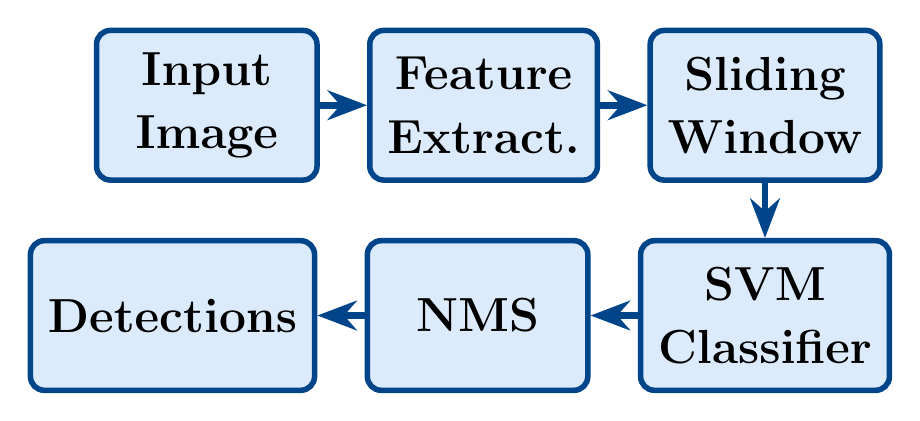
\begin{tikzpicture}[node distance=0.5cm and 0.6cm]
  \node[block] (n1) {Input\\Image};
  \node[block, right=of n1] (n2) {Feature\\Extract.};
  \node[block, right=of n2] (n3) {Sliding\\Window};
  \node[block, below=0.7cm of n3] (n4) {SVM\\Classifier};
  \node[block, left=of n4]  (n5) {NMS};
  \node[block, left=of n5]  (n6) {Detections};
  \draw[arr] (n1) -- (n2);
  \draw[arr] (n2) -- (n3);
  \draw[arr] (n3) -- (n4);
  \draw[arr] (n4) -- (n5);
  \draw[arr] (n5) -- (n6);
\end{tikzpicture}\\[5pt]
{\small\textit{Fig.\,1: Traditional sliding-window detection pipeline.}}
\end{center}

\medskip
\textbf{Limitation:} Hand-crafted features impose a
\emph{representational ceiling} --- unable to capture high-level
semantics across diverse scenes.  This motivated end-to-end learned
feature extraction via deep CNNs (AlexNet, 2012).

%% ═══════════════════════════════ COLUMN 2 ════════════════════════════════ %%
\columnbreak

\sechead{METHODS \& ARCHITECTURES}

{\large\bfseries Two-Stage Detectors}

\smallskip
R-CNN (2014) $\to$ Fast R-CNN (2015) $\to$
\textbf{Faster R-CNN (2015).}  A learned \textbf{Region Proposal
Network} (RPN) generates object candidates on a shared CNN feature
map; an RoI-Pooling head classifies and refines each proposal.
\emph{Strong mAP; moderate FPS due to sequential stages.}

\begin{center}
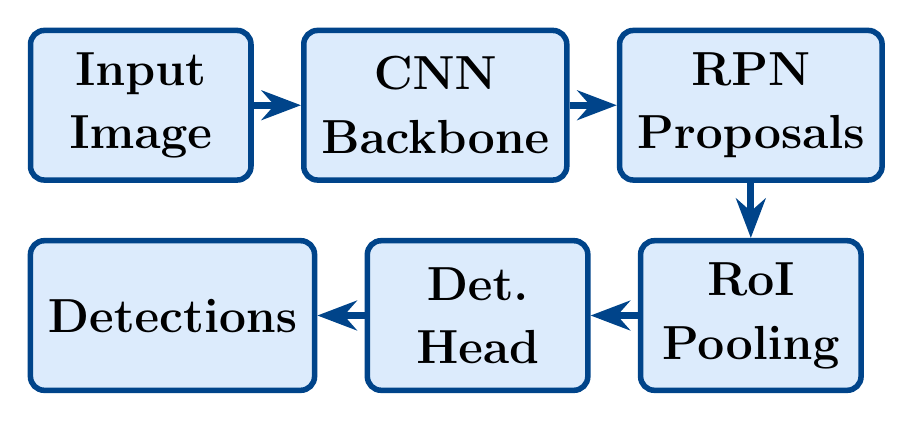
\begin{tikzpicture}[node distance=0.5cm and 0.6cm]
  \node[block] (n1) {Input\\Image};
  \node[block, right=of n1] (n2) {CNN\\Backbone};
  \node[block, right=of n2] (n3) {RPN\\Proposals};
  \node[block, below=0.7cm of n3] (n4) {RoI\\Pooling};
  \node[block, left=of n4]  (n5) {Det.\\Head};
  \node[block, left=of n5]  (n6) {Detections};
  \draw[arr] (n1) -- (n2);
  \draw[arr] (n2) -- (n3);
  \draw[arr] (n3) -- (n4);
  \draw[arr] (n4) -- (n5);
  \draw[arr] (n5) -- (n6);
\end{tikzpicture}\\[5pt]
{\small\textit{Fig.\,2: Two-stage detection pipeline (Faster R-CNN).}}
\end{center}

\medskip
{\large\bfseries One-Stage Detectors}

\smallskip
YOLO (2016)\,/\,SSD (2016)\,/\,RetinaNet (2017) predict class scores
and box offsets \textbf{directly at every spatial location} in a
single forward pass.  \textbf{Focal Loss} solved the extreme
foreground--background imbalance:
\[
  \mathrm{FL}(p_t)=-\alpha_t(1-p_t)^{\gamma}\log(p_t)
\]

\begin{center}
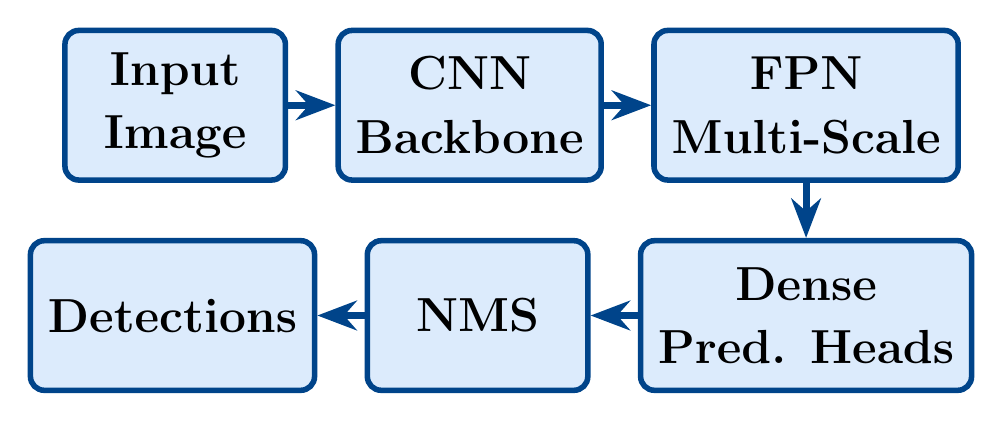
\begin{tikzpicture}[node distance=0.5cm and 0.6cm]
  \node[block] (n1) {Input\\Image};
  \node[block, right=of n1] (n2) {CNN\\Backbone};
  \node[block, right=of n2] (n3) {FPN\\Multi-Scale};
  \node[block, below=0.7cm of n3] (n4) {Dense\\Pred. Heads};
  \node[block, left=of n4]  (n5) {NMS};
  \node[block, left=of n5]  (n6) {Detections};
  \draw[arr] (n1) -- (n2);
  \draw[arr] (n2) -- (n3);
  \draw[arr] (n3) -- (n4);
  \draw[arr] (n4) -- (n5);
  \draw[arr] (n5) -- (n6);
\end{tikzpicture}\\[5pt]
{\small\textit{Fig.\,3: One-stage pipeline (YOLO\,/\,SSD\,/\,RetinaNet).}}
\end{center}

\medskip
{\large\bfseries DETR: Transformer Set Prediction}

\smallskip
DETR (2020) replaces RPN, RoI Pooling, and NMS with a
\textbf{transformer encoder--decoder} and \textbf{bipartite
(Hungarian) matching}.  It directly predicts an unordered \emph{set}
of object hypotheses --- no hand-designed post-processing required.
Swin Transformer (2021) introduced hierarchical windowed attention for
efficient multi-scale detection.

\begin{center}
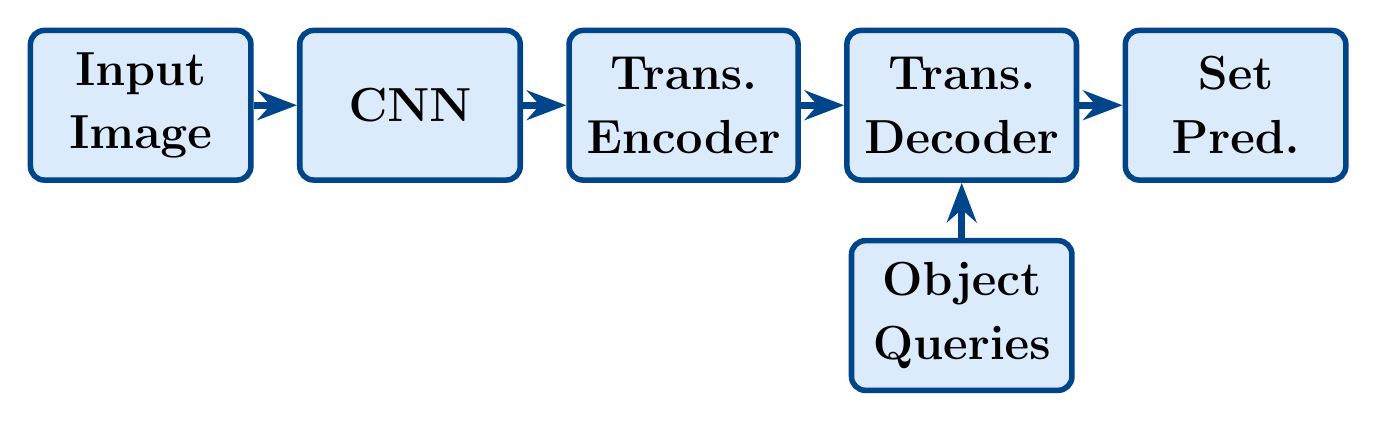
\begin{tikzpicture}[node distance=0.45cm and 0.55cm]
  \node[block] (img) {Input\\Image};
  \node[block, right=of img] (cnn) {CNN};
  \node[block, right=of cnn] (enc) {Trans.\\Encoder};
  \node[block, right=of enc] (dec) {Trans.\\Decoder};
  \node[block, right=of dec] (out) {Set\\Pred.};
  \node[block, below=0.7cm of dec] (oq) {Object\\Queries};
  \draw[arr] (img) -- (cnn);
  \draw[arr] (cnn) -- (enc);
  \draw[arr] (enc) -- (dec);
  \draw[arr] (dec) -- (out);
  \draw[arr] (oq)  -- (dec);
\end{tikzpicture}\\[5pt]
{\small\textit{Fig.\,4: DETR pipeline (no anchors, no NMS required).}}
\end{center}

%% ═══════════════════════════════ COLUMN 3 ════════════════════════════════ %%
\columnbreak

\sechead{COMPARATIVE INSIGHTS}

\begin{center}
\small
\setlength{\tabcolsep}{0.6em}
\renewcommand{\arraystretch}{1.4}
\begin{tabular}{lcccc}
\toprule
\textbf{Model} & \textbf{mAP} & \textbf{FPS} & \textbf{GFLOPs} &
  \textbf{Params (M)} \\
\midrule
Faster R-CNN & 42.0 & 26  & 246 & 60.1 \\
SSD512       & 29.8 & 61  &  90 & 26.3 \\
DETR         & 42.0 & 38  &  86 & 41.3 \\
YOLOv8-L     & 46.8 & 97  & 165 & 43.7 \\
\bottomrule
\end{tabular}\\[6pt]
{\footnotesize\textit{COCO-style reference metrics (single-GPU).}}
\end{center}

\begin{center}
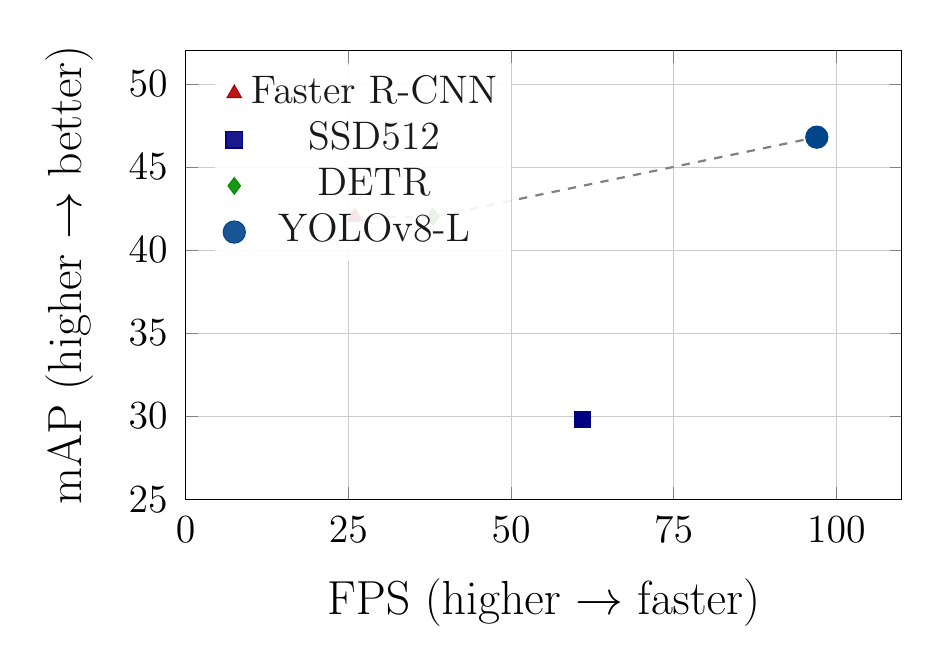
\begin{tikzpicture}
\begin{axis}[
  width=0.88\columnwidth, height=0.60\columnwidth,
  grid=both,
  grid style={line width=.1pt, draw=gray!25},
  major grid style={line width=.2pt, draw=gray!40},
  xlabel={\small FPS (higher $\to$ faster)},
  ylabel={\small mAP (higher $\to$ better)},
  xmin=0, xmax=110, ymin=25, ymax=52,
  xtick={0,25,50,75,100},
  ytick={25,30,35,40,45,50},
  ticklabel style={font=\footnotesize},
  label style={font=\small},
  legend style={
    font=\footnotesize,
    at={(0.04,0.97)}, anchor=north west,
    draw=none, fill=white, fill opacity=0.9},
]
\addplot[only marks, mark=triangle*, mark size=3pt, color=red!70!black]
  coordinates {(26,42.0)};
\addlegendentry{Faster R-CNN}
\addplot[only marks, mark=square*, mark size=3pt, color=blue!50!black]
  coordinates {(61,29.8)};
\addlegendentry{SSD512}
\addplot[only marks, mark=diamond*, mark size=3pt, color=green!55!black]
  coordinates {(38,42.0)};
\addlegendentry{DETR}
\addplot[only marks, mark=*, mark size=4pt, color=posterblue]
  coordinates {(97,46.8)};
\addlegendentry{YOLOv8-L}
\addplot[thick, dashed, color=black!50]
  coordinates {(26,42.0)(38,42.0)(97,46.8)};
\end{axis}
\end{tikzpicture}\\[5pt]
{\small\textit{Fig.\,5: Pareto frontier --- accuracy vs.\ throughput.\\
  Dashed line\,=\,illustrative efficiency frontier.}}
\end{center}

\sechead{CONCLUSION}

Object detection evolved from hand-crafted sliding-window pipelines to
deep two-stage proposal networks, one-stage dense predictors, and
transformer-based set prediction.  Each generation navigated the
\textbf{speed--accuracy trade-off} differently:
\begin{itemize}[nosep, leftmargin=*]
  \item Two-stage designs maximised mAP through staged refinement.
  \item One-stage designs maximised FPS via dense prediction and
    improved training objectives.
  \item Transformers (DETR) eliminated hand-designed post-processing,
    enabling fully end-to-end learnable detection.
\end{itemize}

\medskip
No single ``best'' architecture exists: the optimal design is
deployment-specific, balancing latency budgets, hardware constraints,
and accuracy--efficiency trade-offs.  Emerging directions --- Edge AI,
3D detection, and open-vocabulary grounding --- will further reshape
this frontier.

\sechead{REFERENCES}

\begin{enumerate}[nosep, leftmargin=*, label={[\arabic*]}]
\small
\item P.\,Viola \& M.\,Jones, CVPR 2001.
\item N.\,Dalal \& B.\,Triggs, CVPR 2005.
\item P.\,Felzenszwalb et\,al., TPAMI 2010.
\item R.\,Girshick et\,al.\ (R-CNN), CVPR 2014.
\item R.\,Girshick (Fast R-CNN), ICCV 2015.
\item S.\,Ren et\,al.\ (Faster R-CNN), NeurIPS 2015.
\item J.\,Redmon et\,al.\ (YOLO), CVPR 2016.
\item W.\,Liu et\,al.\ (SSD), ECCV 2016.
\item T.-Y.\,Lin et\,al.\ (Focal Loss), ICCV 2017.
\item N.\,Carion et\,al.\ (DETR), ECCV 2020.
\item Z.\,Liu et\,al.\ (Swin), ICCV 2021.
\item G.\,Jocher et\,al.\ (YOLOv8), 2023.
\end{enumerate}

\end{multicols}
\end{document}
